\documentclass[tikz,border=3mm]{standalone}
\usepackage{tikz}
\usetikzlibrary{angles,quotes,calc,intersections}
\begin{document}
% TikZ 1
\begin{tikzpicture}[scale=.75]
\draw[->,thick] (-4.5,0)--(4.5,0) node[right] {$x$};
\draw[->,thick] (0,-4.5)--(0,4.5) node[above] {$y$};
\foreach \x in {-4,-3,-2,-1,1,2,3,4}{\draw (\x,.08)--(\x,-.08) node[below] {$\x$};}
\foreach \y in {-4,-3,-2,-1,1,2,3,4}{\draw (.08,\y)--(-.08,\y) node[left] {$\y$};}
\node[below left] at (0,0) {$O$};
\node at (2.8,2.8) {I};
\node at (-2.8,2.8) {II};
\node at (-2.8,-2.8) {III};
\node at (2.8,-2.8) {IV};
\end{tikzpicture}
\hspace{1cm}
% TikZ 2
\begin{tikzpicture}[scale=.8]
\draw[->,thick] (-1,0)--(7,0) node[right] {$x$};
\draw[->,thick] (0,-1)--(0,5) node[above] {$y$};
\coordinate (A) at (0,0); \coordinate (B) at (6,4); \coordinate (M) at (3,2);
\draw[thick,blue!70!black] (A)--(B);
\fill (A) circle (2pt) node[below left] {$A$};
\fill (B) circle (2pt) node[above right] {$B$};
\fill (M) circle (2pt) node[above left] {$M$};
\end{tikzpicture}

\vspace{1cm}

% TikZ 3
\begin{tikzpicture}[scale=.8]
\draw[->,thick] (-1,0)--(7,0) node[right] {$x$};
\draw[->,thick] (0,-1)--(0,5) node[above] {$y$};
\coordinate (A) at (1,1); \coordinate (B) at (6,4); \coordinate (C) at (6,1);
\draw[thick,blue!70!black] (A)--(B);
\draw[thick,dashed] (A)--(C)--(B);
\pic[draw=blue!70!black, angle radius=4mm] {right angle=A--C--B};
\node[below] at ($(A)!0.5!(C)$) {$\Delta x$};
\node[right] at ($(C)!0.5!(B)$) {$\Delta y$};
\fill (A) circle (2pt) node[below left] {$A$};
\fill (B) circle (2pt) node[above right] {$B$};
\end{tikzpicture}
\hspace{1cm}
% TikZ 4
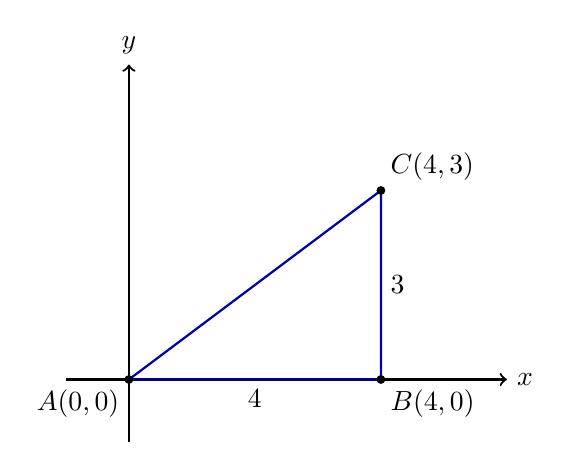
\begin{tikzpicture}[scale=.8]
\draw[->,thick] (-1,0)--(6,0) node[right] {$x$};
\draw[->,thick] (0,-1)--(0,5) node[above] {$y$};
\coordinate (A) at (0,0); \coordinate (B) at (4,0); \coordinate (C) at (4,3);
\draw[thick,blue!70!black] (A)--(B)--(C)--cycle;
\fill (A) circle (2pt) node[below left] {$A(0,0)$};
\fill (B) circle (2pt) node[below right] {$B(4,0)$};
\fill (C) circle (2pt) node[above right] {$C(4,3)$};
\node[below] at (2,0) {$4$};
\node[right] at (4,1.5) {$3$};
\end{tikzpicture}
\end{document}
